\section{Architektur}

\subsection{Model-View-Controller}
Die Grundstruktur der Webanwendung orientiert sich an der "Model View Controller"-Architektur. Die Aufteilung der Webanwendung in diese 3 Komponenten entkoppelt unser Datenmodell von seiner Darstellung und erleichtert daher die nachträgliche Erweiterung bzw. Veränderung der Anwendung.
Die drei Komponenten sollen dabei folgende Aufgaben erfüllen:
\begin{addmargin}[25pt]{0pt}
    \textbf{Model}\\
    Das Model enthält die Datenstruktur der Messtationen, angelehnt an die Datenstruktur des \gls{FROST-Server}s, und für die Objekte der Karte.
    \\ \\
    \textbf{Controller}\\
    Der Controller ist die zentrale Steuerungseinheit der Webanwendung. Er entscheidet was bei Nutzereingaben passieren soll und kümmert sich darum Daten vom \gls{FROST-Server} abzurufen und den REACT-Komponenten in passender Form zur Darstellung zu übergeben,
    \\ \\
    \textbf{View}\\
    Die View kümmert sich über \gls{React} um die Interaktion mit dem Benutzer. Sie zeigt die Detail- und MapPage an, und nimmt ebenfalls Interaktionen des Benutzers entgegen und leitet diese an den Controller weiter.
\end{addmargin}

Des Weiteren wird der Code entsprechend dem Entwurfsprinzip "separation of concerns" nach Aufgaben getrennt. Somit wird der Programmcode logisch strukturiert und bleibt übersichtlich und verständlich. Das erleichtert auch die gemeinsame Entwicklung im Team.

\vspace{5mm}

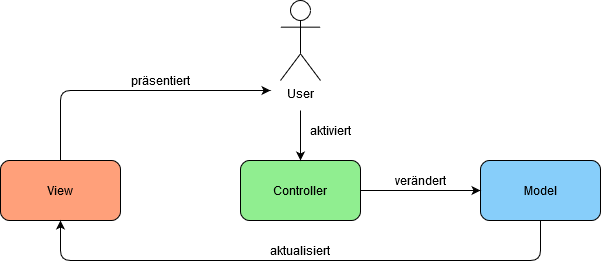
\includegraphics[width=\textwidth,keepaspectratio]{MVC_Pattern.png}

\newpage

\subsection{Datenfluss über eine Fassade}
Ein weiterer Punkt auf den wir beim Entwurf besonders geachtet haben ist der Datenfluss unserer Webanwendung. Da wir unsere Daten von einem externen Server beziehen, der nicht in unserer Hand liegt, müssen wir alle ankommenden Daten zuerst verifizieren und in unser Datenmodell überführen. Des Weiteren sind Anfragen an den externen Server unter umständen komplex und müssen in mehrere Teilanfragen zerlegt werden.
Da eigentlich alle Komponenten unserer Webanwendung externe Daten benötigen, haben wir uns entschieden, Anfragen, Verifizierung und die Adaption der Daten an unser Datenmodell an eine eigene Komponente (FROST-package) auszulagern. Die Kommunikation mit anderen Programmteilen erfolgt über eine Fassadenklasse.

Hierdurch ergeben sich folgende Vorteile:
\begin{itemize}
    \item Daten werden hinter der Fassade verifiziert, vor der Fassade kann die Konsistenz der Daten vorrausgesetzt werden und muss nicht nochmal überprüft werden
    \item Programmcode zur Formulierung von Anfragen, Verifizierung der Daten und Überführung in unsere Model-Objekte muss nur an einer Stelle implementiert werden
    \item Programmcode kann leichter ergänzt werden (z.B. Möglichkeit zum Cachen großer Anfragen an einer zentralen Stelle hinter der Fassade)
    \item Gemäß dem Geheimnisprinzip wird die ursprüngliche Form der Daten hinter der Fassade verborgen
\end{itemize}

\vspace{5mm}

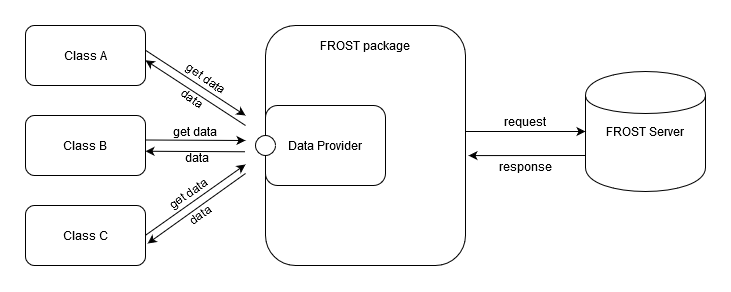
\includegraphics[width=\textwidth,keepaspectratio]{Facade_Pattern.png}
